%% LyX 1.5.6 created this file.  For more info, see http://www.lyx.org/.
%% Do not edit unless you really know what you are doing.
\documentclass[ngerman]{scrartcl}
\usepackage[T1]{fontenc}
\usepackage[latin9]{inputenc}
\setlength{\parskip}{\medskipamount}
\setlength{\parindent}{0pt}
\usepackage{graphicx}
\usepackage{babel}

\begin{document}

\part*{Religion}


\section*{04.02.09}


\subsection*{Motivationen f�r soziales Handeln?}

\begin{itemize}
\item Gut sein wollen
\item religi�s
\item sich hineinversetzen, Mitleid, Mitgef�hl
\item Wertsch�tzung bekommen
\item Dank bekommen
\item menschlich sein / menschlicher werden
\item Vertrauen, Freundschaft
\item Spa�
\item Sorge um andere Menschen
\item geschwisterliche Verbundenheit
\item Ver�nderung der Gesellschaft
\item Verantwortung wahrnehmen
\item Erfahrungen sammeln
\item das Leben sch�tzen lernen
\end{itemize}

\subsection*{Biblische Erfahrungen}

Einstieg: Mk 1, 14-15 in verschiedenen �bersetzungen

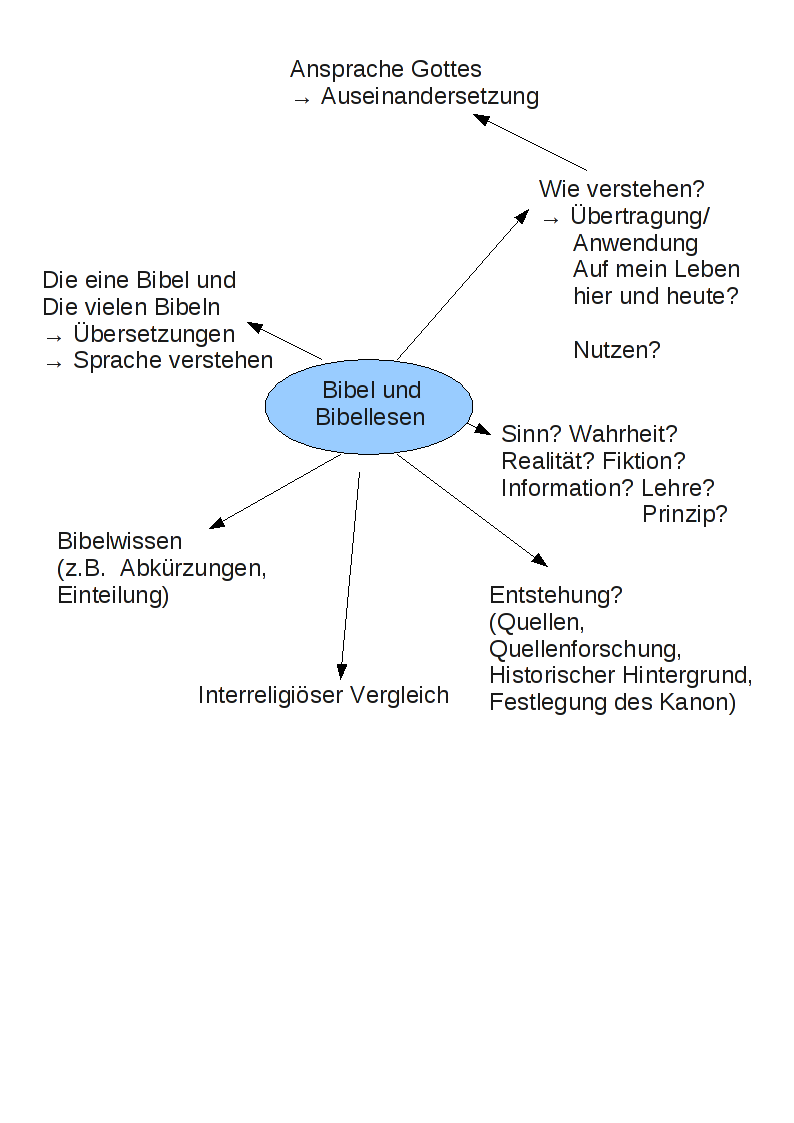
\includegraphics[scale=0.7]{Mindmap1}
\end{document}
